\documentclass[11pt]{exam}

\usepackage{amsmath}
\usepackage{graphicx}
\usepackage{geometry}
\usepackage{etoolbox}
\BeforeBeginEnvironment{choices}{\par\nopagebreak\minipage{\linewidth}}
\AfterEndEnvironment{choices}{\endminipage}
\geometry{
a4paper,
total={185mm,257mm},
left=10mm,
top=25mm,
bottom=10mm
}

\begin{document}
\setlength{\voffset}{-0.5in}
\setlength{\headsep}{5pt}

\fbox{\fbox{\parbox{8cm}{\centering
\vspace{2mm}
Testat - Versuch E - Diffusion und Osmose - 1
\vspace{2mm}
}}}
\hspace{2mm}
\makebox[0.25\textwidth]{Name:\enspace\hrulefill} \hspace{5mm}
\makebox[0.2\textwidth]{Datum:\enspace\hrulefill}
\vspace{4mm}

\begin{questions}

\question Die Leitfähigkeit von 15 ml Salzlösung wird zu 4,4 \( \frac{\mu S}{cm} \) bestimmt. Diese Salzlösung wird nun mit destilliertem Wasser auf 60 ml aufgefüllt. Welche Leitfähigkeit wird nun gemessen?

\begin{choices}
	\choice 8,8 \(   \frac{\mu S}{cm}  \)
	\choice 3,3 \(   \frac{\mu S}{cm}  \)
	\choice 1,1 \(   \frac{\mu S}{cm}  \)
	\choice 2,2 \(   \frac{\mu S}{cm}  \)
	\choice 4,4 \(   \frac{\mu S}{cm}  \)
\end{choices}

\vspace{3mm}\question Wo ist der Konzentrationsgradient der schwarzen Teilchen über die Membran (grau) am größten? 

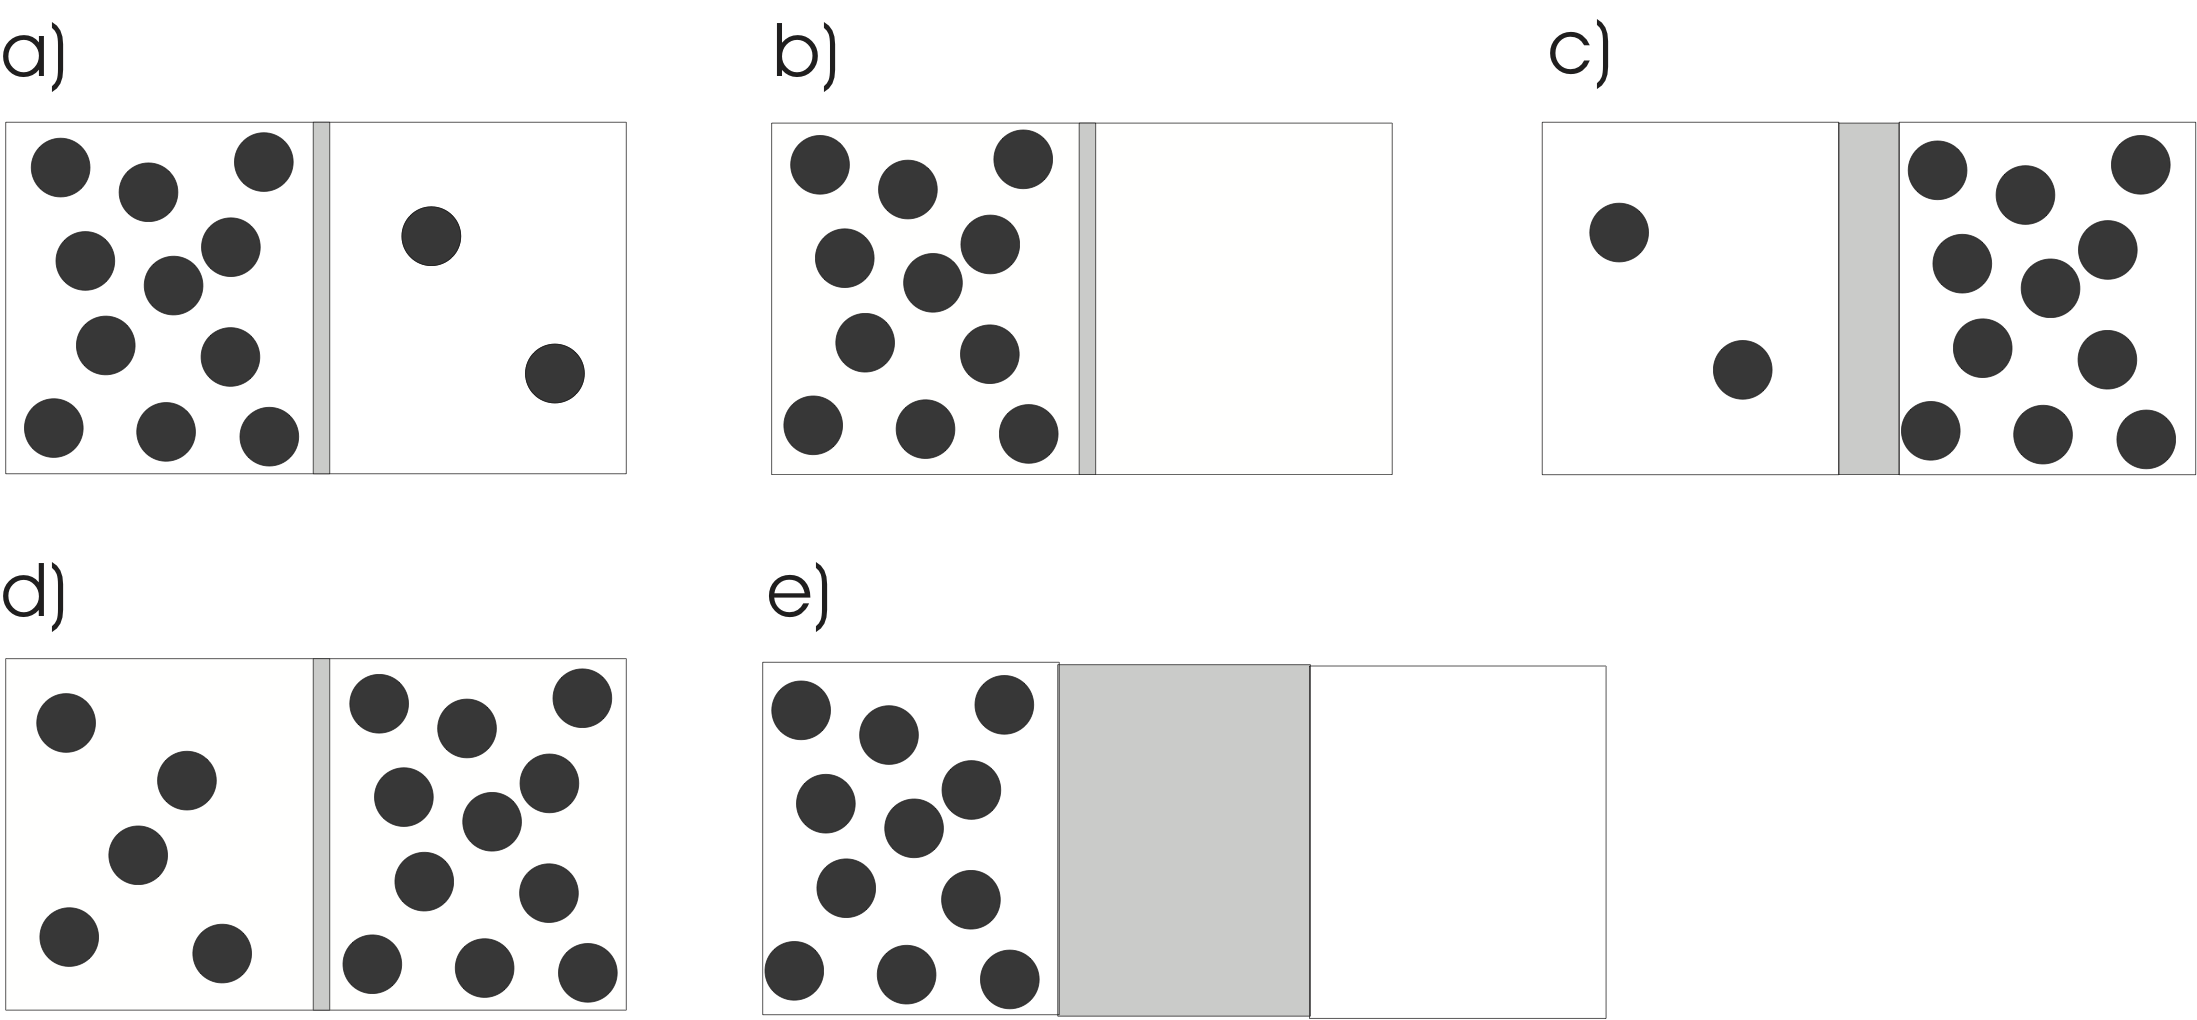
\includegraphics[width=0.5\textwidth]{../../../questions/E/images/Diffusion.png}

\begin{choices}
	\choice e)
	\choice b)
	\choice c)
	\choice a)
	\choice d)
\end{choices}

\vspace{3mm}\question Wie ändert sich der Diffusionsfluss \( J \) durch eine kreisförmige Membran, wenn deren Durchmesser sich verdoppelt?

\begin{choices}
	\choice \( J \) vervierfacht sich.
	\choice \( J \) verdoppelt sich.
	\choice \( J \) halbiert sich.
	\choice \( J \) ist unabhängig vom Durchmesser der Membran.
	\choice \( J \) quadriert sich.
\end{choices}

\vspace{3mm}\question Der Diffusionsfluss beschreibt ...

\begin{choices}
	\choice die transportierte Stoffmenge pro Volumen.
	\choice die transportierte Stoffmenge.
	\choice die transportierte Stoffmenge pro Zeit.
	\choice die transportierte Stoffmenge pro Fläche.
	\choice die transportierte Stoffmenge pro Zeit und Fläche.
\end{choices}

\vspace{3mm}\question Was ist die SI-Einheit des Diffusionskoeffizienten?

\begin{choices}
	\choice \( \frac{kg \cdot m^2}{s} \)
	\choice \( \frac{s}{m^2} \)
	\choice \( \frac{m^3}{s} \)
	\choice \( \frac{kg}{s} \)
	\choice \( \frac{m^2}{s} \)
\end{choices}

\vspace{3mm}\end{questions}

\end{document}
